\documentclass[submission]{eptcs}
\providecommand{\event}{VSS 2025} % Name of the event you are submitting to

% VSS 2025: International Workshop on Verification of Scientific Software
% May 4, 2025     Hamilton ON, Canada
% https://vsl.cis.udel.edu/vss2025/
\usepackage{iftex}

\usepackage{listings}
\usepackage{xcolor}
\usepackage{graphicx}

\lstset{
    basicstyle=\ttfamily\small,
    keywordstyle=\color{blue}\bfseries,
    commentstyle=\color{gray},
    stringstyle=\color{red},
    breaklines=true
}

\ifpdf
  \usepackage{underscore}         % Only needed if you use pdflatex.
  \usepackage[T1]{fontenc}        % Recommended with pdflatex
\else
  \usepackage{breakurl}           % Not needed if you use pdflatex only.
\fi

\title{Verification Challenges in Sparse Matrix Vector Multiplication in High Performance Computing}
\author{Junchao Zhang
\institute{Argonne National Laboratory, Illinois, USA}
\email{jczhang@anl.gov}
}
\def\titlerunning{Verification challenges in SpMV in HPC}
\def\authorrunning{J. Zhang}
\begin{document}
\maketitle

\begin{abstract}
Sparse matrix vector multiplication is a crucial kernel in scientific codes
using iterative solvers. We present a sequential and a basic MPI parallel implementations of
the kernel on the CPU, to provide challenges to the scientific software verification community.
We describle the implementations
in the context of the PETSc library.
\end{abstract}

\section{Introduction}
Solving sparse linear systems of $Ax=b$ lies in the heart of scientific computing.
Iterative Krylov subspace methods \cite{saad2003iterative} are a key algorithm for that,
especially for large scale computations.
In Krylov methods, sparse matrix vector multiplication (SpMV) is a crucial kernel.
The popular math library, PETSc (the Portable, Extensible Toolkit for Scientific Computation)\cite{petsc-user-ref}, contains
a suite of Krylov methods and SpMV implementations.
% which are the backbone of PETSc's higher layer algorithms such as non-linear sovlers, time-steppers and optimizers.
% These iterative methods approximate the solution $x_m$ from a subspace $x_0 + span\{r_0,\ Ar_0,\ A^2r_0,\ ...,\ A^{m-1}r_0\}$
% with $x_0$ representing an arbitrary initial guess to the solution and $r_0=b-Ax_0$.
% The equation $A^kr = A \cdot (A^{k-1}r)$ implies the importance of matrix vector multiplication for the methods.
Since the matrix is usually very sparse,
it is wise to only store nonzeros to save memory.
The compressed sparse row (CSR), known as {\tt MATAIJ} in PETSc,
is a commonly used sparse matrix storage format.
It represents an {\tt m} $\times$ {\tt n} matrix with total {\tt nnz} nozeros in three arrays: {\tt a[nnz]}, {\tt i[m]} and {\tt j[nnz]},
 where {\tt a[]} and {\tt j[]} store the nonzeros and their column indices row-wisely, respectively, and {\tt i[]}
stores indices pointing to the start of each row in {\tt a[]} and {\tt j[]}.
Apparently, {\tt i[0] = 0} and row {\tt k} has {\tt i[k+1] - i[k]} nonzeros. {\tt i[m]} points to the next place
after the last nonzero. Figure \ref{fig:seqcsr} shows a CSR example for a 4 $\times$ 12 sparse matrix.

\begin{figure}[h]
  \centering
  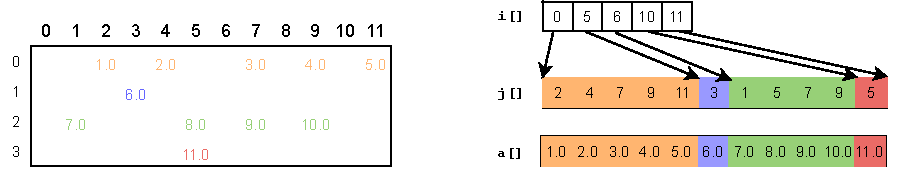
\includegraphics[width=0.8\textwidth]{figs/SEQCSR.pdf}
  \caption{{\it Left}: A 4 $\times$ 12 sparse matrix. {\it Right}:  its compressed sparse row (CSR) representation.}
  \label{fig:seqcsr}
\end{figure}

Matrix vector multplication has a very simple definition.
Denote $A = \{a_{ij}\}$, $x = \{x_j\}$, $y = \{y_i\}$, then $y = Ax$ defines
$y_i = \sum_{j=0}^{n-1}a_{ij} x_j$, with $0\leq i < m$, $0 \leq j < n$.
However, it is the storage format, data distribution, parallelization and optimizations
that make implementations complicated.
PETSc has many SpMV implementations.
Among them there is an MPI parallel implementation on the CPU with sophiscated optimizations.
We won't elaborate that one here.
Instead, we present a sequential and an MPI basic implementations, which are simple but still share good
ingredients with the MPI optimized one.
% to give the verfication community an easy start.
We first describle the structure of the code, then the two implementations and the verification challenges within. We conclude at the end.

\section{Code structure, input and output}
We provide standalone implementations written in the C language in a
public repository\footnote{\url{https://github.com/jczhang07/cs2}}.
One only needs to specify a C compiler or an MPI compiler to compile.
The input data is hardwired in source code with global varibles.
We provide matrix $A$ of size {\tt M} $\times$ {\tt N} and {\tt NNZ} nonzeros in three arrays
{\tt Gi[M+1]}, {\tt Gj[NNZ]}, {\tt Ga[NNZ]},
vector $x$ in {\tt Xa[N]}, and the correct answer $z = Ax$ in {\tt Za[M]}. There is also an array {\tt Ya[M]}
to provide space for vector $y$, which will store the computed result of $Ax$. The code will compute the square of
the 2-norm of $|| y - z ||$, which should be zero, and return a non-zero code if $y$ is incorrect.
The input data was generated by the accompanied Python script csr.py. One can modify parameters in the script and re-run
it to generate a different set of input.


\section{Sequential implementation}
\label{sec:seq}
In this implementation (seq.c), marix $A$, vectors $x$, $y$ and $z$ reside in one process.
% They correspond to PETSc's {\tt MATSEQAIJ} and {\tt VECSEQ} types respectively.
We directly build $A$, $x$, $y$ and $z$ from the global arrays mentioned above.
Sizes of $x$, $y$ and $z$ must conform to $A$'s shape.
% The kernel is quite simple, which performs dot product between $A$'s rows and vector $x$ and stores the result in $y$.
% \noindent
\vspace{-10pt}
\begin{figure}[h]
\begin{minipage}{0.35\textwidth}
\begin{lstlisting}[language=C]
typedef struct {
  int     m, n; // size
  int    *i, *j;
  double *a;    // values
} Mat;

typedef struct {
  int     n; // size
  double *a; // values
} Vec;
\end{lstlisting}
\end{minipage}
\hfill
\begin{minipage}{0.55\textwidth}
  \begin{lstlisting}[language=C]
int i, j;
for (i = 0; i < A.m; i++) {
  y.a[i] = 0.0;
  for (j = A.i[i]; j < A.i[i + 1]; j++)
    y.a[i] += A.a[j] * x.a[A.j[j]];
}
\end{lstlisting}
% \vspace{50pt}
\end{minipage}
\vspace{-10pt}
\caption{{\it Left}: sequential matrix and vector types. {\it Right}: sequential SpMV kernel.}
\label{fig:seqcsr}
\vspace{-5pt}
\end{figure}

Figure \ref{fig:seqcsr} shows the sequential matrix and vector types and the SpMV kernel.
We identify these challenges in verifying $y=Ax$ in the code:
\begin{description}
  \item [Challenge 1]: Understand the {\tt Mat} and {\tt Vec} data structures and the CSR format.
  \item [Challenge 2]: Understand the nested loop, array indices, and especially the indirection in {\tt x.a[A.j[j]]}.
\end{description}


\section{MPI basic implementation}
\label{sec:mpibasic}
This implementation (mpibasic.c) uses MPI parallelsim.
The global matrix is block-distributed by row. Each MPI process has a piece (submatrix) of the
matrix, where the row size of the submatrix can be set by users
or automatically computed by PETSc. We call it the matrix row layout.
Though matrix columns are not distrubuted, they also have a layout that can be set by users.
These row and column layouts are properties of the matrix, by which we distribute vectors $y$ and $x$ respectively.
In PETSc, one can use {\tt MatCreateVecs(A, \&x, \&y)} to create
vectors with conforming size and layout suitable for doing $y = Ax$.
We use {\tt M}, {\tt N} to represent the global size of the matrix,
and {\tt m}, {\tt n} for the local size of the diagonal block of the matrix
on this process. {\tt m}, {\tt n} are also the local size of $y$ and $x$ respectively.
In this implementation, we first compute the matrix layouts.
Suppose {\tt size} is the size of {\tt MPI_COMM_WORLD} and {\tt rank} is the rank of the current MPI process,
{\tt m}, {\tt n} are computed as \verb|m = M/size + (M%size > rank ? 1 : 0)|,
\verb|n = N/size + (N%size > rank ? 1 : 0)|. This is the formula PETSc would use
if users don't set {\tt m} and {\tt n}.
With the layouts set,
each process knows the indices of its first row {\tt rstart} and first column {\tt cstart}.
Then it pulls out its data from the global arrays.
{\tt A.j[]} and {\tt A.a[]} can share the space with {\tt Gi[]} and {\tt Ga[]}, but we
have to allocate {\tt A.i[]} and populate it with shifted indices from {\tt Gi[]}.
Similarily, we can build $x$, $y$ and $z$ by pointing them to
{\tt Xa[cstart]}, {\tt Ya[rstart]} and {\tt Za[rstart]} repectively.


% \noindent
\vspace{-10pt}
\begin{figure}[h]
\begin{minipage}{0.35\textwidth}
\begin{lstlisting}[language=C]
typedef struct {
  int     m, n, M, N;
  int     rstart, cstart;
  int    *i, *j;
  double *a;
} Mat;

typedef struct {
  int     n, N;
  double *a;
} Vec;
\end{lstlisting}
\end{minipage}
\hfill
\begin{minipage}{0.60\textwidth}
    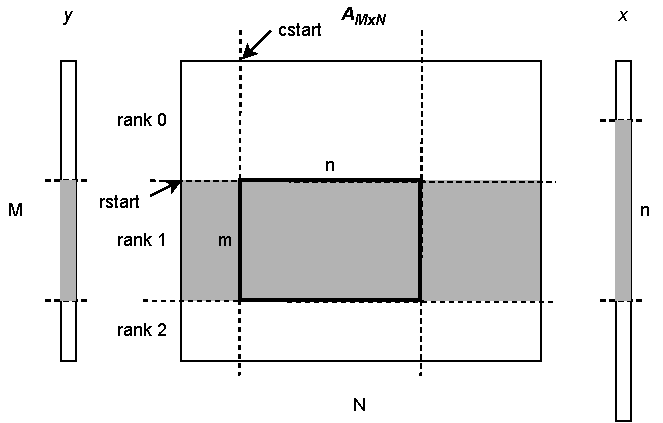
\includegraphics[width=1.0\textwidth]{figs/MPICSR.pdf}
\end{minipage}
\vspace{-10pt}
\caption{{\it Left}: MPI parallel matrix and vector types.
{\it Right}: distributed matrix $A$ and vectors $x$ and $y$ on three MPI ranks.
The shadowed parts reside on rank 1.}
\label{fig:mpicsr}
\vspace{-5pt}
\end{figure}


To multiply the local submatrix $A$ with vector $x$, we need remote entries of $x$. In theory, we only
need entries of $x$ which corresponds to nonzero columns in the local submatrix. But for simplicity,
we gather the whole distributed $x$ to a local vector $X$ of size {\tt N}.
Depending on whether {\tt N} is evenly distributed or not, we can use {\tt MPI_Allgather} or {\tt MPI_Allgatherv}.
With our block distribution formula, this can be tested by {\tt N\%size}. Otherwise,
one has to check whether all {\tt n}'s on processes are equal.
With $X$, we perform a sequential SpMV as in Section \ref{sec:seq} and get the local part of
$y$. After that we compute the partial norm of $||y - z||$, and
then the final norm with the help of {\tt MPI_Allreduce}.
We identify these extra challenges in verifying $y=Ax$ in this MPI basic SpMV:

\begin{description}
  \item [Challenge 3]: Understand the matrix and vector distribution and their size conformity.
  \item [Challenge 4]: Understand the all gather operation on $x$.
  % \item [Challenge 5]: Understand the {\tt MPI_Reduce} operation getting the final norm of $||y - z||$.
\end{description}

\section{Conclusion and future work}
We described a sequential and an MPI basic implementations of the SpMV kernel
in the context of the PETSc library, provided standalone C code and identified
some challenges for the scientifc software verfication community.
In the future, we'd like to add other variants,
such as the MPI optimized implementation used by PETSc, and GPU implementations, to make the challenge code closer to real code.

\nocite{*}
\bibliographystyle{eptcs}
\bibliography{refs.bib}
\end{document}
